\subsection{Vehicle measurements}
\label{sec:vehicle}

During this last measurement, we wanted to test our converter under
the conditions of in vivo vehicle measurements. The great advantage in
this setting is, that all European guidelines for Nitrogen Oxide
emission only talk about \ch{NO_x} (c.\,f.~\cite{eu}), i.\,e.\ in this
case we do not need to separate \ch{NO2} from \ch{NO}. Still we wanted
to compare our \ch{NO_x} results to the results of pure \ch{NO2}
measurements to gauge the influence of the additional \ch{NO} on the
air pollution. Therefore we decided to use two cavities in
parallel. One with our converter, the other one without. With this
very comfortable setup, we could even compute the \ch{NO}
concentration without having to switch the Ozone, which mitigated all
the undesired effects described in the previous two sections.

\subsubsection{Setup}
\label{sec:vehicle-setup}

For the measurement we loaded a car (Ford Focus) with both cavities
and positioned the pickup tube directly above the front license
plate. The \ch{NO_x} cavity was setup according to
Section~\ref{sec:inclusion} with an exposure time of
\SI{10}{\milli\second} and 1000 scans per spectrum leading to a time
resolution of \SI{1}{\second}. As \ch{NO2}
cavity we used the AQM$_{\text{Tec}}$ Compact Cavity, which is the
standard cavity at the Institute for Environmental Physics for
measurements in urban areas and especially vehicle measurements. This
cavity operated at a \SI{2}{\second} timely resolution. The
measurement took place on Friday, February 05, 2016 in Heidelberg
between 11:00 and 16:30. From 12:15 to 13:45, we operated both
cavities in \ch{NO2} mode to test for systematic deviations. From
15:00 to 16:15, we positioned our measurement car next to the
Heidelberg air quality measurement station to be able to compare our
\ch{NO} and \ch{NO2} values to the ones of the station as a measure of
reliability. In between we followed various vehicles throughout
Heidelberg between {\nfrac{} 1/2}~\si{\minute} and \SI{10}{\minute}
and tried to stay within their exhaust plume. Since the two cavities's
clocks could not be fully synchronized, the timeseries had to be
matched in the evaluation step. This was done manually using succinct
peaks in the plots.
\todo{write something about \ch{CO2}}

\begin{figure}[htbp]
  \centering
  % GNUPLOT: LaTeX picture with Postscript
\begingroup
  \makeatletter
  \providecommand\color[2][]{%
    \GenericError{(gnuplot) \space\space\space\@spaces}{%
      Package color not loaded in conjunction with
      terminal option `colourtext'%
    }{See the gnuplot documentation for explanation.%
    }{Either use 'blacktext' in gnuplot or load the package
      color.sty in LaTeX.}%
    \renewcommand\color[2][]{}%
  }%
  \providecommand\includegraphics[2][]{%
    \GenericError{(gnuplot) \space\space\space\@spaces}{%
      Package graphicx or graphics not loaded%
    }{See the gnuplot documentation for explanation.%
    }{The gnuplot epslatex terminal needs graphicx.sty or graphics.sty.}%
    \renewcommand\includegraphics[2][]{}%
  }%
  \providecommand\rotatebox[2]{#2}%
  \@ifundefined{ifGPcolor}{%
    \newif\ifGPcolor
    \GPcolorfalse
  }{}%
  \@ifundefined{ifGPblacktext}{%
    \newif\ifGPblacktext
    \GPblacktexttrue
  }{}%
  % define a \g@addto@macro without @ in the name:
  \let\gplgaddtomacro\g@addto@macro
  % define empty templates for all commands taking text:
  \gdef\gplbacktext{}%
  \gdef\gplfronttext{}%
  \makeatother
  \ifGPblacktext
    % no textcolor at all
    \def\colorrgb#1{}%
    \def\colorgray#1{}%
  \else
    % gray or color?
    \ifGPcolor
      \def\colorrgb#1{\color[rgb]{#1}}%
      \def\colorgray#1{\color[gray]{#1}}%
      \expandafter\def\csname LTw\endcsname{\color{white}}%
      \expandafter\def\csname LTb\endcsname{\color{black}}%
      \expandafter\def\csname LTa\endcsname{\color{black}}%
      \expandafter\def\csname LT0\endcsname{\color[rgb]{1,0,0}}%
      \expandafter\def\csname LT1\endcsname{\color[rgb]{0,1,0}}%
      \expandafter\def\csname LT2\endcsname{\color[rgb]{0,0,1}}%
      \expandafter\def\csname LT3\endcsname{\color[rgb]{1,0,1}}%
      \expandafter\def\csname LT4\endcsname{\color[rgb]{0,1,1}}%
      \expandafter\def\csname LT5\endcsname{\color[rgb]{1,1,0}}%
      \expandafter\def\csname LT6\endcsname{\color[rgb]{0,0,0}}%
      \expandafter\def\csname LT7\endcsname{\color[rgb]{1,0.3,0}}%
      \expandafter\def\csname LT8\endcsname{\color[rgb]{0.5,0.5,0.5}}%
    \else
      % gray
      \def\colorrgb#1{\color{black}}%
      \def\colorgray#1{\color[gray]{#1}}%
      \expandafter\def\csname LTw\endcsname{\color{white}}%
      \expandafter\def\csname LTb\endcsname{\color{black}}%
      \expandafter\def\csname LTa\endcsname{\color{black}}%
      \expandafter\def\csname LT0\endcsname{\color{black}}%
      \expandafter\def\csname LT1\endcsname{\color{black}}%
      \expandafter\def\csname LT2\endcsname{\color{black}}%
      \expandafter\def\csname LT3\endcsname{\color{black}}%
      \expandafter\def\csname LT4\endcsname{\color{black}}%
      \expandafter\def\csname LT5\endcsname{\color{black}}%
      \expandafter\def\csname LT6\endcsname{\color{black}}%
      \expandafter\def\csname LT7\endcsname{\color{black}}%
      \expandafter\def\csname LT8\endcsname{\color{black}}%
    \fi
  \fi
    \setlength{\unitlength}{0.0500bp}%
    \ifx\gptboxheight\undefined%
      \newlength{\gptboxheight}%
      \newlength{\gptboxwidth}%
      \newsavebox{\gptboxtext}%
    \fi%
    \setlength{\fboxrule}{0.5pt}%
    \setlength{\fboxsep}{1pt}%
\begin{picture}(7776.00,4320.00)%
    \gplgaddtomacro\gplbacktext{%
      \csname LTb\endcsname%
      \put(682,440){\makebox(0,0)[r]{\strut{}$10$}}%
      \put(682,892){\makebox(0,0)[r]{\strut{}$20$}}%
      \put(682,1344){\makebox(0,0)[r]{\strut{}$30$}}%
      \put(682,1796){\makebox(0,0)[r]{\strut{}$40$}}%
      \put(682,2248){\makebox(0,0)[r]{\strut{}$50$}}%
      \put(682,2699){\makebox(0,0)[r]{\strut{}$60$}}%
      \put(682,3151){\makebox(0,0)[r]{\strut{}$70$}}%
      \put(682,3603){\makebox(0,0)[r]{\strut{}$80$}}%
      \put(682,4055){\makebox(0,0)[r]{\strut{}$90$}}%
      \put(814,220){\makebox(0,0){\strut{}12:10}}%
      \put(1471,220){\makebox(0,0){\strut{}12:20}}%
      \put(2127,220){\makebox(0,0){\strut{}12:30}}%
      \put(2784,220){\makebox(0,0){\strut{}12:40}}%
      \put(3440,220){\makebox(0,0){\strut{}12:50}}%
      \put(4097,220){\makebox(0,0){\strut{}13:00}}%
      \put(4753,220){\makebox(0,0){\strut{}13:10}}%
      \put(5410,220){\makebox(0,0){\strut{}13:20}}%
      \put(6066,220){\makebox(0,0){\strut{}13:30}}%
      \put(6723,220){\makebox(0,0){\strut{}13:40}}%
      \put(7379,220){\makebox(0,0){\strut{}13:50}}%
    }%
    \gplgaddtomacro\gplfronttext{%
      \csname LTb\endcsname%
      \put(176,2247){\rotatebox{-270}{\makebox(0,0){\strut{}Concentration [ppb]}}}%
      \csname LTb\endcsname%
      \put(6392,3882){\makebox(0,0)[r]{\strut{}\text{\ch{NO2} of ICAD \ch{NO2} CE-DOAS}}}%
      \csname LTb\endcsname%
      \put(6392,3662){\makebox(0,0)[r]{\strut{}\text{\ch{NO2} of ICAD \ch{NO_x} CE-DOAS}}}%
    }%
    \gplbacktext
    \put(0,0){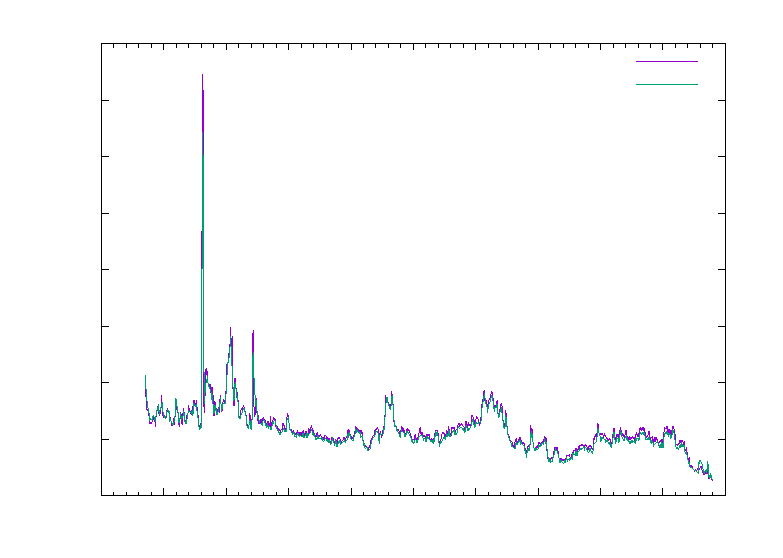
\includegraphics{../images/hd_comparison}}%
    \gplfronttext
  \end{picture}%
\endgroup

  \caption{Comparison of the two used CE-DOAS systems. Both were
    operated in pure \ch{NO2} measurement mode. The difference is
    \SI{0.43 \pm 0.01}{ppb}.}
  \label{fig:hd-comparison}
\end{figure}

\subsubsection{Results}
\label{sec:vehicle-results}

In Figure~\ref{fig:hd-comparison} you can see the comparison of the
measured \ch{NO2} concentrations of the two used cavities. It is
clearly visible that ther is no qualitative difference between the
two. However, our \ch{NO_x} cavity measures slightly lower
concentrations than the \ch{NO2} cavity with a mean difference of
$\Delta = \SI{0.43\pm0.01}{ppb}$. Absolutely speaking this is not a
large difference, but the question remains why it shows up at all. The
most probable explanation is that the used zero air spectrum of the
\ch{NO_x} cavity was not completely trace gas free. On reason that
points towards this direction is, that in the \ch{NO_x} measurement
mode, we have a constant flow through the zero air input, as this is
the input for the Ozone generator. Thus the zero air filters are much
more strained than they would be in a cavity without \ch{NO_x}
mode. Additionally the cavity had been thoroughly tested for multiple
weeks, such that a saturation or starting effects of a saturation of
the Silica gel or the activated carbon seem plausible. 

\begin{figure}[htbp]
  \centering
  % GNUPLOT: LaTeX picture with Postscript
\begingroup
  \makeatletter
  \providecommand\color[2][]{%
    \GenericError{(gnuplot) \space\space\space\@spaces}{%
      Package color not loaded in conjunction with
      terminal option `colourtext'%
    }{See the gnuplot documentation for explanation.%
    }{Either use 'blacktext' in gnuplot or load the package
      color.sty in LaTeX.}%
    \renewcommand\color[2][]{}%
  }%
  \providecommand\includegraphics[2][]{%
    \GenericError{(gnuplot) \space\space\space\@spaces}{%
      Package graphicx or graphics not loaded%
    }{See the gnuplot documentation for explanation.%
    }{The gnuplot epslatex terminal needs graphicx.sty or graphics.sty.}%
    \renewcommand\includegraphics[2][]{}%
  }%
  \providecommand\rotatebox[2]{#2}%
  \@ifundefined{ifGPcolor}{%
    \newif\ifGPcolor
    \GPcolorfalse
  }{}%
  \@ifundefined{ifGPblacktext}{%
    \newif\ifGPblacktext
    \GPblacktexttrue
  }{}%
  % define a \g@addto@macro without @ in the name:
  \let\gplgaddtomacro\g@addto@macro
  % define empty templates for all commands taking text:
  \gdef\gplbacktext{}%
  \gdef\gplfronttext{}%
  \makeatother
  \ifGPblacktext
    % no textcolor at all
    \def\colorrgb#1{}%
    \def\colorgray#1{}%
  \else
    % gray or color?
    \ifGPcolor
      \def\colorrgb#1{\color[rgb]{#1}}%
      \def\colorgray#1{\color[gray]{#1}}%
      \expandafter\def\csname LTw\endcsname{\color{white}}%
      \expandafter\def\csname LTb\endcsname{\color{black}}%
      \expandafter\def\csname LTa\endcsname{\color{black}}%
      \expandafter\def\csname LT0\endcsname{\color[rgb]{1,0,0}}%
      \expandafter\def\csname LT1\endcsname{\color[rgb]{0,1,0}}%
      \expandafter\def\csname LT2\endcsname{\color[rgb]{0,0,1}}%
      \expandafter\def\csname LT3\endcsname{\color[rgb]{1,0,1}}%
      \expandafter\def\csname LT4\endcsname{\color[rgb]{0,1,1}}%
      \expandafter\def\csname LT5\endcsname{\color[rgb]{1,1,0}}%
      \expandafter\def\csname LT6\endcsname{\color[rgb]{0,0,0}}%
      \expandafter\def\csname LT7\endcsname{\color[rgb]{1,0.3,0}}%
      \expandafter\def\csname LT8\endcsname{\color[rgb]{0.5,0.5,0.5}}%
    \else
      % gray
      \def\colorrgb#1{\color{black}}%
      \def\colorgray#1{\color[gray]{#1}}%
      \expandafter\def\csname LTw\endcsname{\color{white}}%
      \expandafter\def\csname LTb\endcsname{\color{black}}%
      \expandafter\def\csname LTa\endcsname{\color{black}}%
      \expandafter\def\csname LT0\endcsname{\color{black}}%
      \expandafter\def\csname LT1\endcsname{\color{black}}%
      \expandafter\def\csname LT2\endcsname{\color{black}}%
      \expandafter\def\csname LT3\endcsname{\color{black}}%
      \expandafter\def\csname LT4\endcsname{\color{black}}%
      \expandafter\def\csname LT5\endcsname{\color{black}}%
      \expandafter\def\csname LT6\endcsname{\color{black}}%
      \expandafter\def\csname LT7\endcsname{\color{black}}%
      \expandafter\def\csname LT8\endcsname{\color{black}}%
    \fi
  \fi
    \setlength{\unitlength}{0.0500bp}%
    \ifx\gptboxheight\undefined%
      \newlength{\gptboxheight}%
      \newlength{\gptboxwidth}%
      \newsavebox{\gptboxtext}%
    \fi%
    \setlength{\fboxrule}{0.5pt}%
    \setlength{\fboxsep}{1pt}%
\begin{picture}(7200.00,5040.00)%
    \gplgaddtomacro\gplbacktext{%
      \csname LTb\endcsname%
      \put(814,440){\makebox(0,0)[r]{\strut{}$-10$}}%
      \put(814,922){\makebox(0,0)[r]{\strut{}$0$}}%
      \put(814,1403){\makebox(0,0)[r]{\strut{}$10$}}%
      \put(814,1885){\makebox(0,0)[r]{\strut{}$20$}}%
      \put(814,2367){\makebox(0,0)[r]{\strut{}$30$}}%
      \put(814,2848){\makebox(0,0)[r]{\strut{}$40$}}%
      \put(814,3330){\makebox(0,0)[r]{\strut{}$50$}}%
      \put(814,3812){\makebox(0,0)[r]{\strut{}$60$}}%
      \put(814,4293){\makebox(0,0)[r]{\strut{}$70$}}%
      \put(814,4775){\makebox(0,0)[r]{\strut{}$80$}}%
      \put(946,220){\makebox(0,0){\strut{}14:50}}%
      \put(1597,220){\makebox(0,0){\strut{}15:00}}%
      \put(2248,220){\makebox(0,0){\strut{}15:10}}%
      \put(2898,220){\makebox(0,0){\strut{}15:20}}%
      \put(3549,220){\makebox(0,0){\strut{}15:30}}%
      \put(4200,220){\makebox(0,0){\strut{}15:40}}%
      \put(4851,220){\makebox(0,0){\strut{}15:50}}%
      \put(5501,220){\makebox(0,0){\strut{}16:00}}%
      \put(6152,220){\makebox(0,0){\strut{}16:10}}%
      \put(6803,220){\makebox(0,0){\strut{}16:20}}%
    }%
    \gplgaddtomacro\gplfronttext{%
      \csname LTb\endcsname%
      \put(176,2607){\rotatebox{-270}{\makebox(0,0){\strut{}Concentration [ppb]}}}%
      \csname LTb\endcsname%
      \put(5816,4602){\makebox(0,0)[r]{\strut{}\ch{NO2}}}%
      \csname LTb\endcsname%
      \put(5816,4382){\makebox(0,0)[r]{\strut{}\ch{NO_x}}}%
      \csname LTb\endcsname%
      \put(5816,4162){\makebox(0,0)[r]{\strut{}\ch{NO_{\text{\hphantom{x}}}}}}%
    }%
    \gplbacktext
    \put(0,0){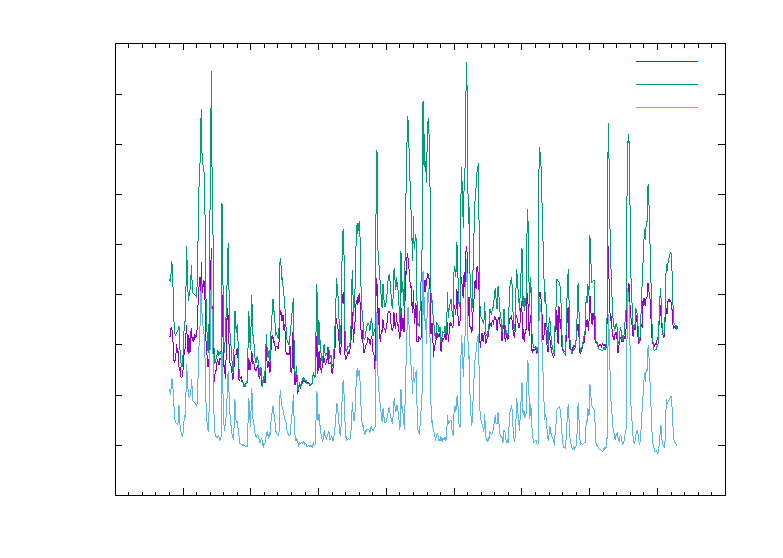
\includegraphics{../images/umba_ts}}%
    \gplfronttext
  \end{picture}%
\endgroup

  \caption{Timeseries of the \ch{NO_x}, \ch{NO2} and the computed
    \ch{NO} concentration next to the Umweltlandesamt air quality
    measurement station in Heidelberg.}
  \label{fig:umba}
\end{figure}

Figure~\ref{fig:umba} contains the timeseries of the measured
\ch{NO_x} and \ch{NO_2} and the computed \ch{NO} during our stay next
to the Heidelberg air quality measurement station. This time series is
representative for all the measurements we took that day. For moderate
\ch{NO2} concentrations between \num{10} and \SI{20}{ppb} the
\ch{NO_x} curve almost coincides with the \ch{NO2} curve. Only during
peaks we have a stronger separation and the \ch{NO_x} concentration
rises occasionally twice as high as the \ch{NO2} concentration. The
time series makes clear that neglecting \ch{NO} values while
estimating \ch{NO_x} pollution in urban areas can lead to
underestimation.

In a next step we computed the average concentrations for all three
time series and compared them to the station data taken
from~\cite{umba}. The results can be found in Table~\ref{tab:umba}. We
see that we have a systematic deviation from the station values,
but our values lie in the same region. The standard CE-DOAS method has
been thoroughly tested during the last decades and is known to produce
solid results ind good accordance with the measurement station. Thus
the deviation of the \ch{NO2} averages already points towards outer
influences, which can explain the deviations. Indeed our pickup tube
was about \SI{3}{\meter} away from the station inlet and approximately
\SI{1}{\meter} lower (which means also closer to the driving
surface). These differences in exact location can easily account for
our measured derivations.

Nevertheless, the main result stays that under field conditions in
ambient air our measured \ch{NO_x} or respectively computed \ch{NO}
values are comparable to the ones of the station, thus indicating once
more that our converter together with a second cavity seem to work as
a good setup for \ch{NO} measurements. Still some more (and longer)
measurements would be advisable to aquire more data points for enough
statistics to make a comparison between the DOAS method and other
established \ch{NO} measurement methods resilient.

\begin{table}[htbp]
  \centering
  \sisetup{
    table-format=2.1(2)
  }
  \begin{tabular}{l S S}
    \toprule
    {Compound} & \multicolumn{2}{c}{Concentration in \si{ppb}}\\
    & {Station} & {DOAS}\\
    \midrule
    \ch{NO} & 7.4 & 6.5 \pm 0.2\\
    \ch{NO2} & 19.2 & 21.9 \pm 0.1\\
    \ch{NOx} & 26.6 & 28.2 \pm 0.4\\ 
    \bottomrule
  \end{tabular}
  \caption{Comparison of the \SI{1}{\hour} \ch{NO}, \ch{NO2} and
    \ch{NO_x} averages from 15:00 to 16:00 on February 05, 2016
    between the air quality measurement station and the improved CE-DOAS
    instrument. The station data was taken from~\cite{umba}; no
    uncertainties were provided.}
  \label{tab:umba}
\end{table}

In between these experiments, we measured \num{30} vehicles within
Heidelberg. The main result is that we have a large discrepancy
between the \ch{NO2} and \ch{NO_x} values. During peaks the \ch{NO_x}
values exceed the \ch{NO2} values by far. Below we discuss two
examples out of these measurements in more detail. First we pursued a
Mercedes B180 CDI.\@ The time series is depicted in
Figure~\ref{fig:mercedes-ts} and a picture of the vehicle together
with the surrounding traffic is shown in Figure~\ref{fig:bus}
left. There are 5 to 6 acceleration
periods visible and most prominent in the \ch{NO_x} time
series. We see that the \ch{NO_2} values vary the least and are
between a factor 4 and a factor 9 smaller than the \ch{NO_x} values
during peaks. In the valleys between peaks, the \ch{NO_x} approaches
the \ch{NO2}, but is still significantly higher. The \ch{CO2} time
series has the same overall appearance as the \ch{NO_x}. If we correct
the concentrations for background pollution and compute averages, we
are able compare the Nitrogen (Di-)Oxide emission to the Carbon
Dioxide emission. This gives us a measure for the pollution per
(gasoline) consumption. The results can be found in
Table~\ref{tab:mercedes-bus}. We find that there is one order of
magnitude difference between the two ratios, which underlines the
blatant underestimation of the vehicle emissions if only \ch{NO2}
values are taken into account.

\begin{figure}[htbp]
  \centering
  % GNUPLOT: LaTeX picture with Postscript
\begingroup
  \makeatletter
  \providecommand\color[2][]{%
    \GenericError{(gnuplot) \space\space\space\@spaces}{%
      Package color not loaded in conjunction with
      terminal option `colourtext'%
    }{See the gnuplot documentation for explanation.%
    }{Either use 'blacktext' in gnuplot or load the package
      color.sty in LaTeX.}%
    \renewcommand\color[2][]{}%
  }%
  \providecommand\includegraphics[2][]{%
    \GenericError{(gnuplot) \space\space\space\@spaces}{%
      Package graphicx or graphics not loaded%
    }{See the gnuplot documentation for explanation.%
    }{The gnuplot epslatex terminal needs graphicx.sty or graphics.sty.}%
    \renewcommand\includegraphics[2][]{}%
  }%
  \providecommand\rotatebox[2]{#2}%
  \@ifundefined{ifGPcolor}{%
    \newif\ifGPcolor
    \GPcolorfalse
  }{}%
  \@ifundefined{ifGPblacktext}{%
    \newif\ifGPblacktext
    \GPblacktexttrue
  }{}%
  % define a \g@addto@macro without @ in the name:
  \let\gplgaddtomacro\g@addto@macro
  % define empty templates for all commands taking text:
  \gdef\gplbacktext{}%
  \gdef\gplfronttext{}%
  \makeatother
  \ifGPblacktext
    % no textcolor at all
    \def\colorrgb#1{}%
    \def\colorgray#1{}%
  \else
    % gray or color?
    \ifGPcolor
      \def\colorrgb#1{\color[rgb]{#1}}%
      \def\colorgray#1{\color[gray]{#1}}%
      \expandafter\def\csname LTw\endcsname{\color{white}}%
      \expandafter\def\csname LTb\endcsname{\color{black}}%
      \expandafter\def\csname LTa\endcsname{\color{black}}%
      \expandafter\def\csname LT0\endcsname{\color[rgb]{1,0,0}}%
      \expandafter\def\csname LT1\endcsname{\color[rgb]{0,1,0}}%
      \expandafter\def\csname LT2\endcsname{\color[rgb]{0,0,1}}%
      \expandafter\def\csname LT3\endcsname{\color[rgb]{1,0,1}}%
      \expandafter\def\csname LT4\endcsname{\color[rgb]{0,1,1}}%
      \expandafter\def\csname LT5\endcsname{\color[rgb]{1,1,0}}%
      \expandafter\def\csname LT6\endcsname{\color[rgb]{0,0,0}}%
      \expandafter\def\csname LT7\endcsname{\color[rgb]{1,0.3,0}}%
      \expandafter\def\csname LT8\endcsname{\color[rgb]{0.5,0.5,0.5}}%
    \else
      % gray
      \def\colorrgb#1{\color{black}}%
      \def\colorgray#1{\color[gray]{#1}}%
      \expandafter\def\csname LTw\endcsname{\color{white}}%
      \expandafter\def\csname LTb\endcsname{\color{black}}%
      \expandafter\def\csname LTa\endcsname{\color{black}}%
      \expandafter\def\csname LT0\endcsname{\color{black}}%
      \expandafter\def\csname LT1\endcsname{\color{black}}%
      \expandafter\def\csname LT2\endcsname{\color{black}}%
      \expandafter\def\csname LT3\endcsname{\color{black}}%
      \expandafter\def\csname LT4\endcsname{\color{black}}%
      \expandafter\def\csname LT5\endcsname{\color{black}}%
      \expandafter\def\csname LT6\endcsname{\color{black}}%
      \expandafter\def\csname LT7\endcsname{\color{black}}%
      \expandafter\def\csname LT8\endcsname{\color{black}}%
    \fi
  \fi
    \setlength{\unitlength}{0.0500bp}%
    \ifx\gptboxheight\undefined%
      \newlength{\gptboxheight}%
      \newlength{\gptboxwidth}%
      \newsavebox{\gptboxtext}%
    \fi%
    \setlength{\fboxrule}{0.5pt}%
    \setlength{\fboxsep}{1pt}%
\begin{picture}(7200.00,5040.00)%
    \gplgaddtomacro\gplbacktext{%
      \csname LTb\endcsname%
      \put(946,966){\makebox(0,0)[r]{\strut{}$0$}}%
      \put(946,1347){\makebox(0,0)[r]{\strut{}$100$}}%
      \put(946,1728){\makebox(0,0)[r]{\strut{}$200$}}%
      \put(946,2109){\makebox(0,0)[r]{\strut{}$300$}}%
      \put(946,2490){\makebox(0,0)[r]{\strut{}$400$}}%
      \put(946,2871){\makebox(0,0)[r]{\strut{}$500$}}%
      \put(946,3251){\makebox(0,0)[r]{\strut{}$600$}}%
      \put(946,3632){\makebox(0,0)[r]{\strut{}$700$}}%
      \put(946,4013){\makebox(0,0)[r]{\strut{}$800$}}%
      \put(946,4394){\makebox(0,0)[r]{\strut{}$900$}}%
      \put(946,4775){\makebox(0,0)[r]{\strut{}$1000$}}%
      \put(1078,834){\rotatebox{-45}{\makebox(0,0)[l]{\strut{}11:15:00}}}%
      \put(1471,834){\rotatebox{-45}{\makebox(0,0)[l]{\strut{}11:15:30}}}%
      \put(1864,834){\rotatebox{-45}{\makebox(0,0)[l]{\strut{}11:16:00}}}%
      \put(2256,834){\rotatebox{-45}{\makebox(0,0)[l]{\strut{}11:16:30}}}%
      \put(2649,834){\rotatebox{-45}{\makebox(0,0)[l]{\strut{}11:17:00}}}%
      \put(3042,834){\rotatebox{-45}{\makebox(0,0)[l]{\strut{}11:17:30}}}%
      \put(3435,834){\rotatebox{-45}{\makebox(0,0)[l]{\strut{}11:18:00}}}%
      \put(3827,834){\rotatebox{-45}{\makebox(0,0)[l]{\strut{}11:18:30}}}%
      \put(4220,834){\rotatebox{-45}{\makebox(0,0)[l]{\strut{}11:19:00}}}%
      \put(4613,834){\rotatebox{-45}{\makebox(0,0)[l]{\strut{}11:19:30}}}%
      \put(5006,834){\rotatebox{-45}{\makebox(0,0)[l]{\strut{}11:20:00}}}%
      \put(5398,834){\rotatebox{-45}{\makebox(0,0)[l]{\strut{}11:20:30}}}%
      \put(5791,834){\rotatebox{-45}{\makebox(0,0)[l]{\strut{}11:21:00}}}%
      \put(5923,966){\makebox(0,0)[l]{\strut{}$0$}}%
      \put(5923,1347){\makebox(0,0)[l]{\strut{}$100$}}%
      \put(5923,1728){\makebox(0,0)[l]{\strut{}$200$}}%
      \put(5923,2109){\makebox(0,0)[l]{\strut{}$300$}}%
      \put(5923,2490){\makebox(0,0)[l]{\strut{}$400$}}%
      \put(5923,2871){\makebox(0,0)[l]{\strut{}$500$}}%
      \put(5923,3251){\makebox(0,0)[l]{\strut{}$600$}}%
      \put(5923,3632){\makebox(0,0)[l]{\strut{}$700$}}%
      \put(5923,4013){\makebox(0,0)[l]{\strut{}$800$}}%
      \put(5923,4394){\makebox(0,0)[l]{\strut{}$900$}}%
      \put(5923,4775){\makebox(0,0)[l]{\strut{}$1000$}}%
    }%
    \gplgaddtomacro\gplfronttext{%
      \csname LTb\endcsname%
      \put(176,2870){\rotatebox{-270}{\makebox(0,0){\strut{}\ch{NO2}/\ch{NO_x} Concentration [ppb]}}}%
      \put(6692,2870){\rotatebox{-270}{\makebox(0,0){\strut{}\ch{CO2} Concentration [ppm]}}}%
      \csname LTb\endcsname%
      \put(4804,4602){\makebox(0,0)[r]{\strut{}\ch{NO2}}}%
      \csname LTb\endcsname%
      \put(4804,4382){\makebox(0,0)[r]{\strut{}\ch{NO_x}}}%
      \csname LTb\endcsname%
      \put(4804,4162){\makebox(0,0)[r]{\strut{}\ch{CO2}}}%
    }%
    \gplbacktext
    \put(0,0){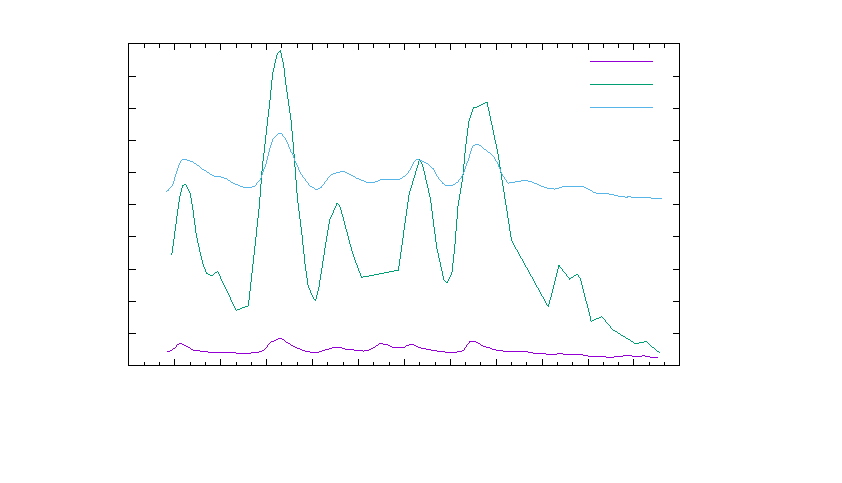
\includegraphics{../images/mercedes}}%
    \gplfronttext
  \end{picture}%
\endgroup

  \caption{Timeseries of the uncorrected \ch{NO2}, \ch{NO_x} and
    \ch{CO2} concentrations in the plume of a VW Pasat TDI.}
  \label{fig:mercedes-ts}
\end{figure}

\begin{figure}[htbp]
  \centering
  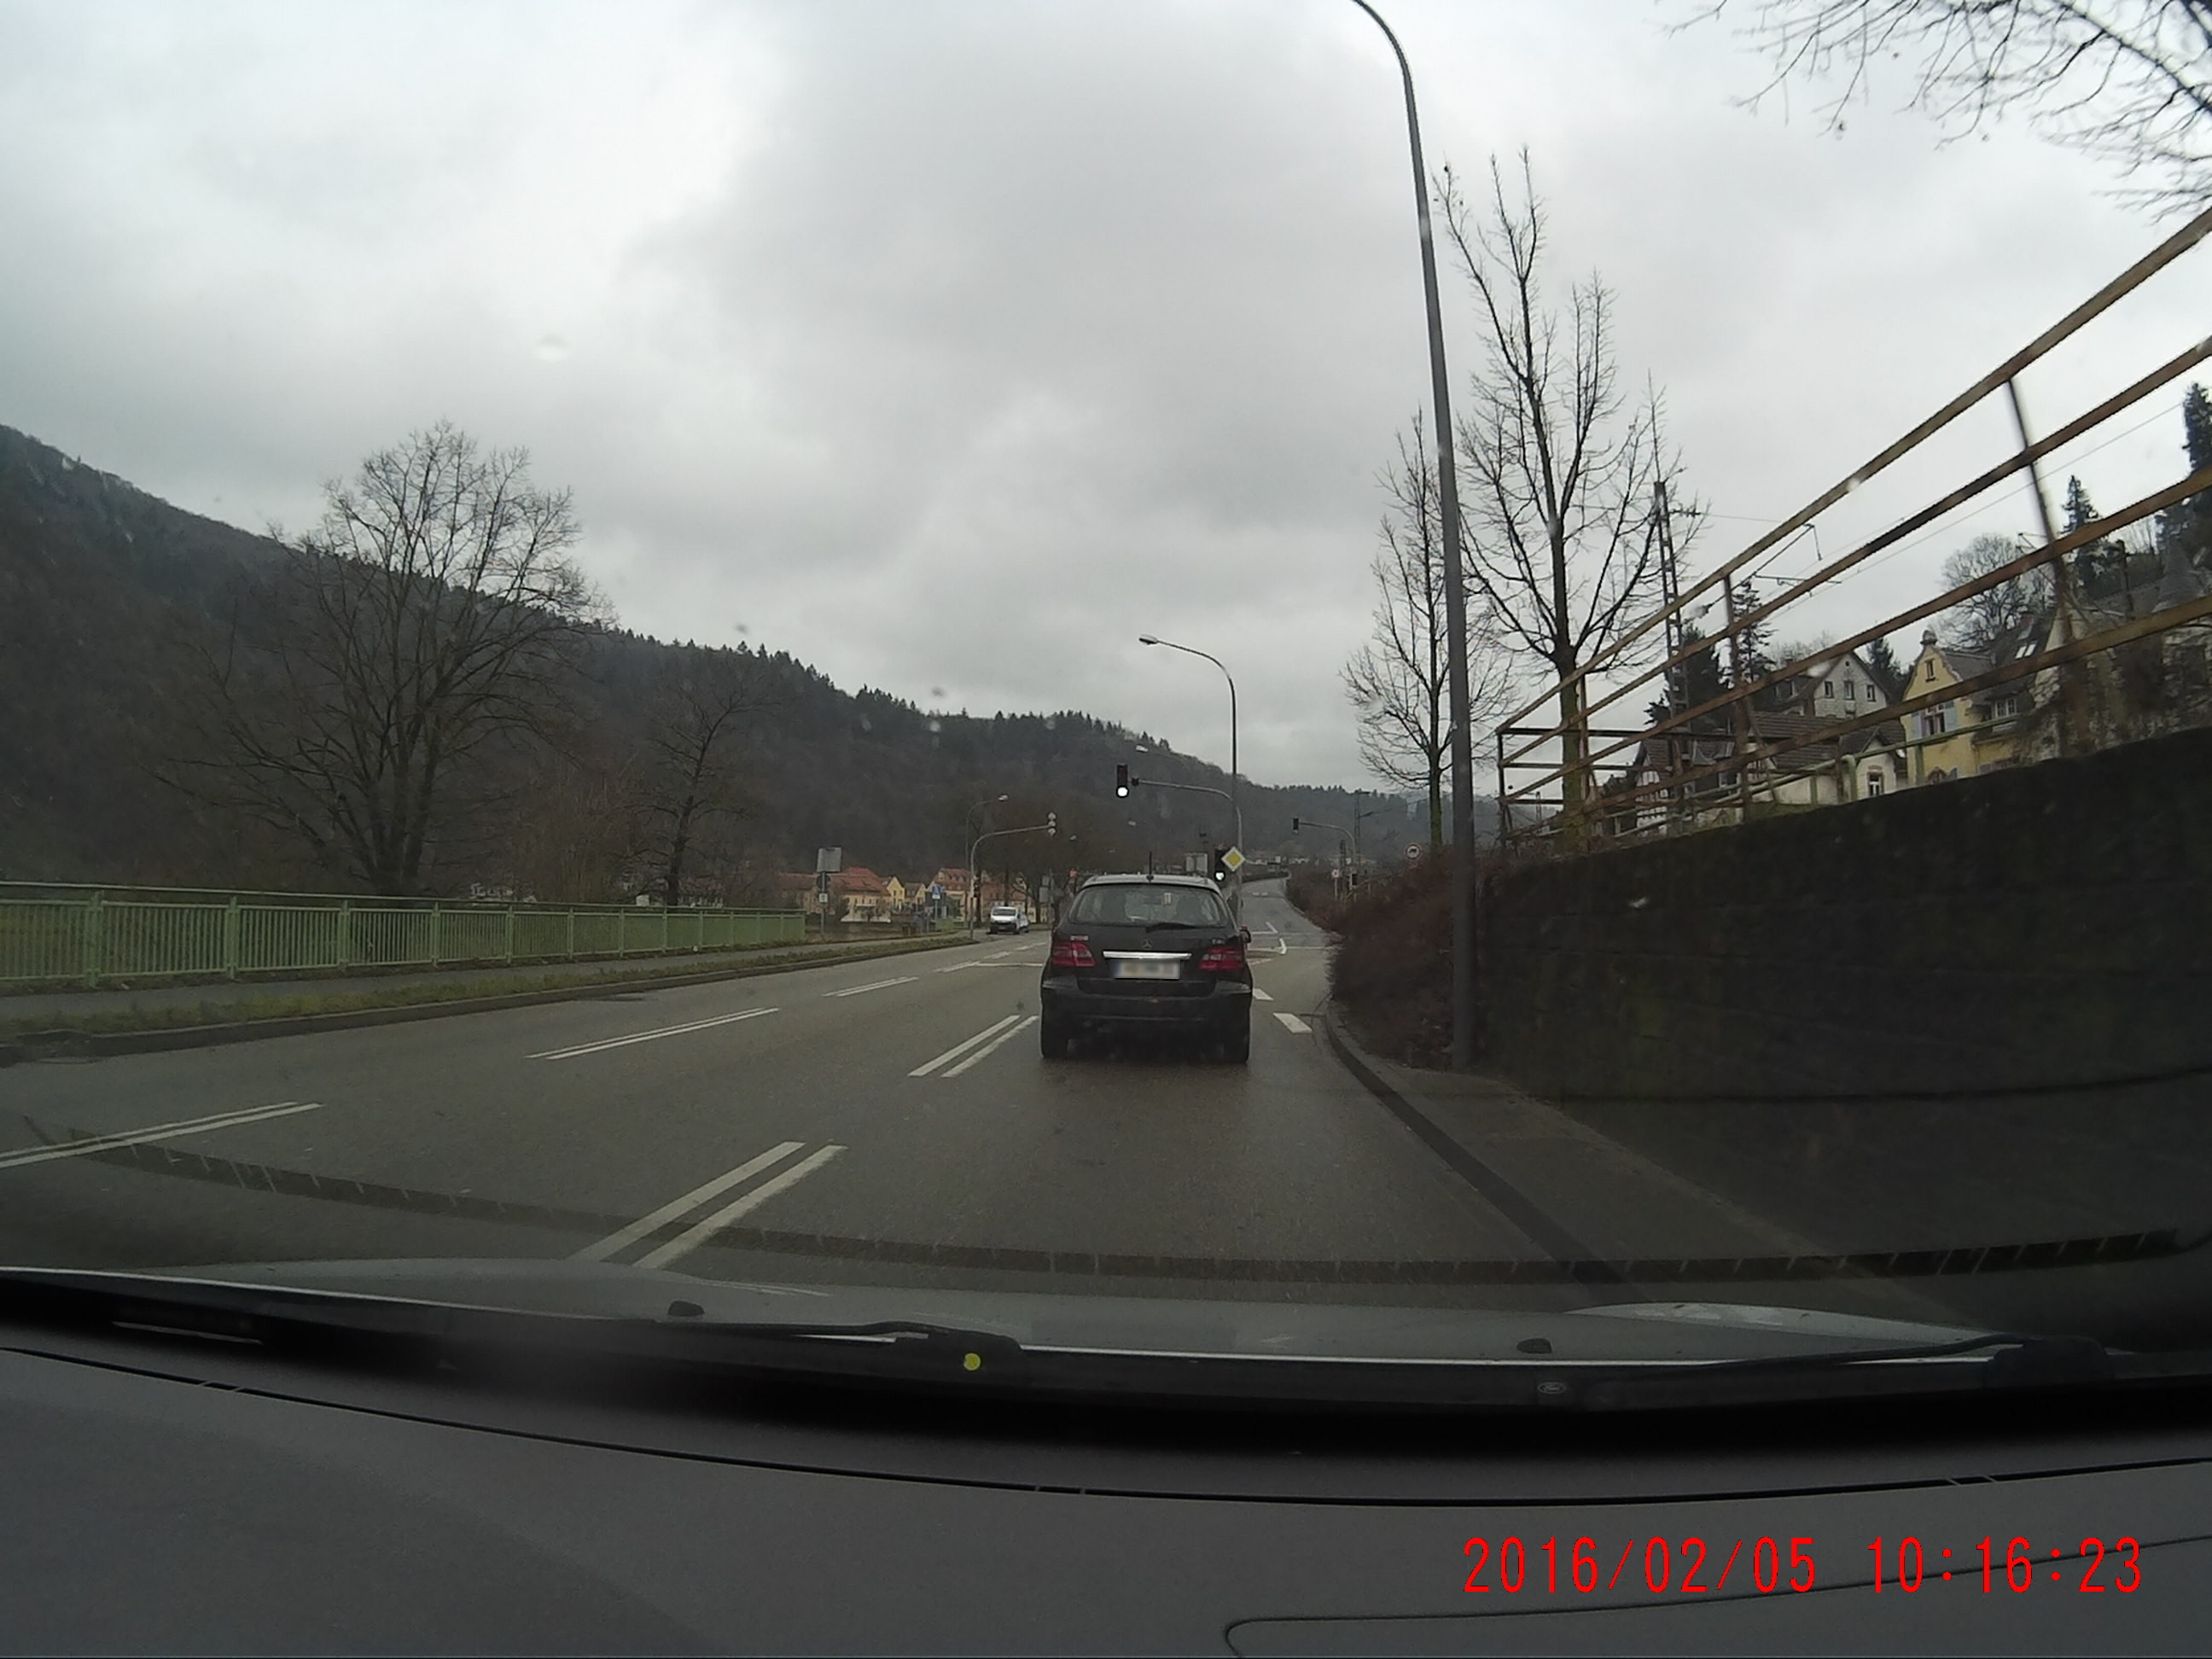
\includegraphics[width=0.45\textwidth]{mercedes.jpg}
  \hfill  
  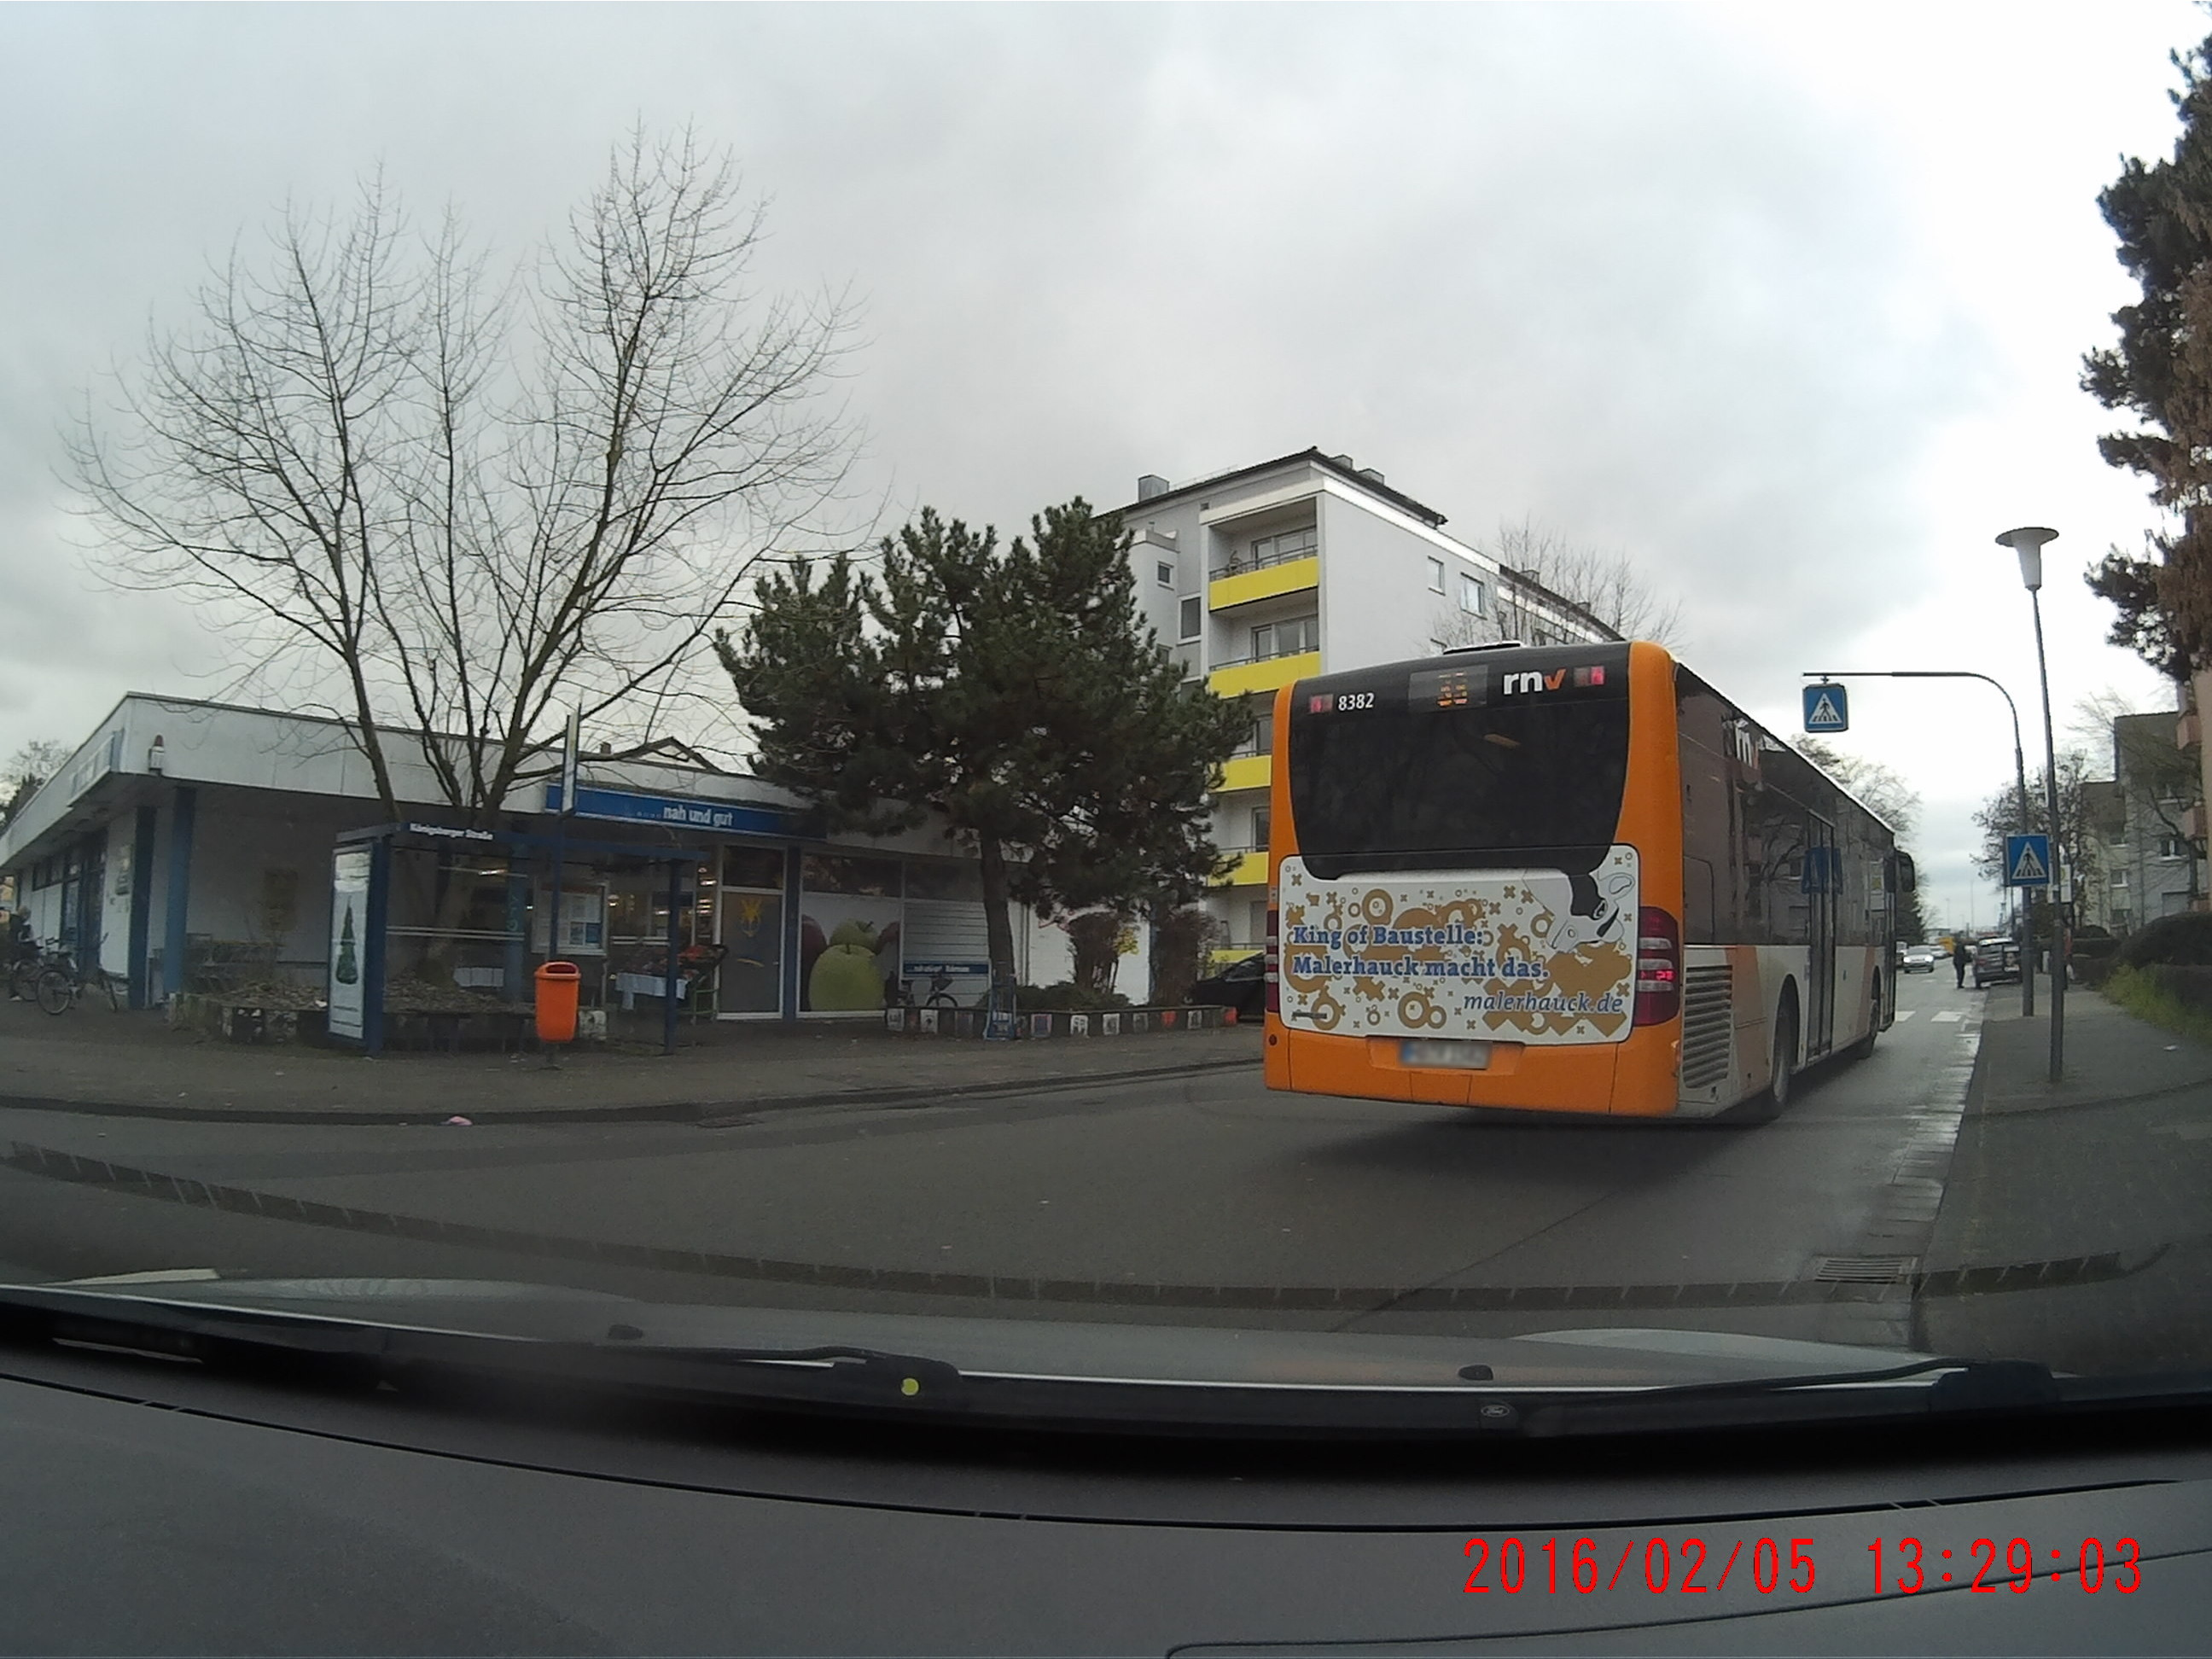
\includegraphics[width=0.45\textwidth]{bus.jpg}
  \caption{Picture of the measured bus and VW Pasat.}
  \label{fig:bus}
\end{figure}

\begin{table}[hbtp]
  \centering
  \begin{tabular}{l S S}
    \toprule
    & {Mercedes} & {Bus}\\
    \midrule
    \ch{NO2}/\ch{CO2} & 2.2(3)e-4 & 6(2)e-4\\
    \ch{NO_x}/\ch{CO2}& 5.0(7)e-3 & 6(1)e-3\\
    \bottomrule
  \end{tabular}
  \caption{\ch{NO2} and \ch{NO_x} to \ch{CO2} ratios for the two
    vehicles.}
  \label{tab:mercedes-bus}
\end{table}

\begin{figure}[htbp]
  \centering
  % GNUPLOT: LaTeX picture with Postscript
\begingroup
  \makeatletter
  \providecommand\color[2][]{%
    \GenericError{(gnuplot) \space\space\space\@spaces}{%
      Package color not loaded in conjunction with
      terminal option `colourtext'%
    }{See the gnuplot documentation for explanation.%
    }{Either use 'blacktext' in gnuplot or load the package
      color.sty in LaTeX.}%
    \renewcommand\color[2][]{}%
  }%
  \providecommand\includegraphics[2][]{%
    \GenericError{(gnuplot) \space\space\space\@spaces}{%
      Package graphicx or graphics not loaded%
    }{See the gnuplot documentation for explanation.%
    }{The gnuplot epslatex terminal needs graphicx.sty or graphics.sty.}%
    \renewcommand\includegraphics[2][]{}%
  }%
  \providecommand\rotatebox[2]{#2}%
  \@ifundefined{ifGPcolor}{%
    \newif\ifGPcolor
    \GPcolorfalse
  }{}%
  \@ifundefined{ifGPblacktext}{%
    \newif\ifGPblacktext
    \GPblacktexttrue
  }{}%
  % define a \g@addto@macro without @ in the name:
  \let\gplgaddtomacro\g@addto@macro
  % define empty templates for all commands taking text:
  \gdef\gplbacktext{}%
  \gdef\gplfronttext{}%
  \makeatother
  \ifGPblacktext
    % no textcolor at all
    \def\colorrgb#1{}%
    \def\colorgray#1{}%
  \else
    % gray or color?
    \ifGPcolor
      \def\colorrgb#1{\color[rgb]{#1}}%
      \def\colorgray#1{\color[gray]{#1}}%
      \expandafter\def\csname LTw\endcsname{\color{white}}%
      \expandafter\def\csname LTb\endcsname{\color{black}}%
      \expandafter\def\csname LTa\endcsname{\color{black}}%
      \expandafter\def\csname LT0\endcsname{\color[rgb]{1,0,0}}%
      \expandafter\def\csname LT1\endcsname{\color[rgb]{0,1,0}}%
      \expandafter\def\csname LT2\endcsname{\color[rgb]{0,0,1}}%
      \expandafter\def\csname LT3\endcsname{\color[rgb]{1,0,1}}%
      \expandafter\def\csname LT4\endcsname{\color[rgb]{0,1,1}}%
      \expandafter\def\csname LT5\endcsname{\color[rgb]{1,1,0}}%
      \expandafter\def\csname LT6\endcsname{\color[rgb]{0,0,0}}%
      \expandafter\def\csname LT7\endcsname{\color[rgb]{1,0.3,0}}%
      \expandafter\def\csname LT8\endcsname{\color[rgb]{0.5,0.5,0.5}}%
    \else
      % gray
      \def\colorrgb#1{\color{black}}%
      \def\colorgray#1{\color[gray]{#1}}%
      \expandafter\def\csname LTw\endcsname{\color{white}}%
      \expandafter\def\csname LTb\endcsname{\color{black}}%
      \expandafter\def\csname LTa\endcsname{\color{black}}%
      \expandafter\def\csname LT0\endcsname{\color{black}}%
      \expandafter\def\csname LT1\endcsname{\color{black}}%
      \expandafter\def\csname LT2\endcsname{\color{black}}%
      \expandafter\def\csname LT3\endcsname{\color{black}}%
      \expandafter\def\csname LT4\endcsname{\color{black}}%
      \expandafter\def\csname LT5\endcsname{\color{black}}%
      \expandafter\def\csname LT6\endcsname{\color{black}}%
      \expandafter\def\csname LT7\endcsname{\color{black}}%
      \expandafter\def\csname LT8\endcsname{\color{black}}%
    \fi
  \fi
    \setlength{\unitlength}{0.0500bp}%
    \ifx\gptboxheight\undefined%
      \newlength{\gptboxheight}%
      \newlength{\gptboxwidth}%
      \newsavebox{\gptboxtext}%
    \fi%
    \setlength{\fboxrule}{0.5pt}%
    \setlength{\fboxsep}{1pt}%
\begin{picture}(7200.00,5040.00)%
    \gplgaddtomacro\gplbacktext{%
      \csname LTb\endcsname%
      \put(946,966){\makebox(0,0)[r]{\strut{}$0$}}%
      \put(946,1389){\makebox(0,0)[r]{\strut{}$500$}}%
      \put(946,1812){\makebox(0,0)[r]{\strut{}$1000$}}%
      \put(946,2236){\makebox(0,0)[r]{\strut{}$1500$}}%
      \put(946,2659){\makebox(0,0)[r]{\strut{}$2000$}}%
      \put(946,3082){\makebox(0,0)[r]{\strut{}$2500$}}%
      \put(946,3505){\makebox(0,0)[r]{\strut{}$3000$}}%
      \put(946,3929){\makebox(0,0)[r]{\strut{}$3500$}}%
      \put(946,4352){\makebox(0,0)[r]{\strut{}$4000$}}%
      \put(946,4775){\makebox(0,0)[r]{\strut{}$4500$}}%
      \put(1078,834){\rotatebox{-45}{\makebox(0,0)[l]{\strut{}14:25:00}}}%
      \put(1549,834){\rotatebox{-45}{\makebox(0,0)[l]{\strut{}14:26:00}}}%
      \put(2021,834){\rotatebox{-45}{\makebox(0,0)[l]{\strut{}14:27:00}}}%
      \put(2492,834){\rotatebox{-45}{\makebox(0,0)[l]{\strut{}14:28:00}}}%
      \put(2963,834){\rotatebox{-45}{\makebox(0,0)[l]{\strut{}14:29:00}}}%
      \put(3435,834){\rotatebox{-45}{\makebox(0,0)[l]{\strut{}14:30:00}}}%
      \put(3906,834){\rotatebox{-45}{\makebox(0,0)[l]{\strut{}14:31:00}}}%
      \put(4377,834){\rotatebox{-45}{\makebox(0,0)[l]{\strut{}14:32:00}}}%
      \put(4848,834){\rotatebox{-45}{\makebox(0,0)[l]{\strut{}14:33:00}}}%
      \put(5320,834){\rotatebox{-45}{\makebox(0,0)[l]{\strut{}14:34:00}}}%
      \put(5791,834){\rotatebox{-45}{\makebox(0,0)[l]{\strut{}14:35:00}}}%
      \put(5923,966){\makebox(0,0)[l]{\strut{}$0$}}%
      \put(5923,1389){\makebox(0,0)[l]{\strut{}$500$}}%
      \put(5923,1812){\makebox(0,0)[l]{\strut{}$1000$}}%
      \put(5923,2236){\makebox(0,0)[l]{\strut{}$1500$}}%
      \put(5923,2659){\makebox(0,0)[l]{\strut{}$2000$}}%
      \put(5923,3082){\makebox(0,0)[l]{\strut{}$2500$}}%
      \put(5923,3505){\makebox(0,0)[l]{\strut{}$3000$}}%
      \put(5923,3929){\makebox(0,0)[l]{\strut{}$3500$}}%
      \put(5923,4352){\makebox(0,0)[l]{\strut{}$4000$}}%
      \put(5923,4775){\makebox(0,0)[l]{\strut{}$4500$}}%
    }%
    \gplgaddtomacro\gplfronttext{%
      \csname LTb\endcsname%
      \put(176,2870){\rotatebox{-270}{\makebox(0,0){\strut{}\ch{NO2}/\ch{NO_x} Concentration [ppb]}}}%
      \put(6692,2870){\rotatebox{-270}{\makebox(0,0){\strut{}\ch{CO2} Concentration [ppm]}}}%
      \csname LTb\endcsname%
      \put(1738,4602){\makebox(0,0)[r]{\strut{}\ch{NO2}}}%
      \csname LTb\endcsname%
      \put(1738,4382){\makebox(0,0)[r]{\strut{}\ch{NO_x}}}%
      \csname LTb\endcsname%
      \put(1738,4162){\makebox(0,0)[r]{\strut{}\ch{CO2}}}%
    }%
    \gplbacktext
    \put(0,0){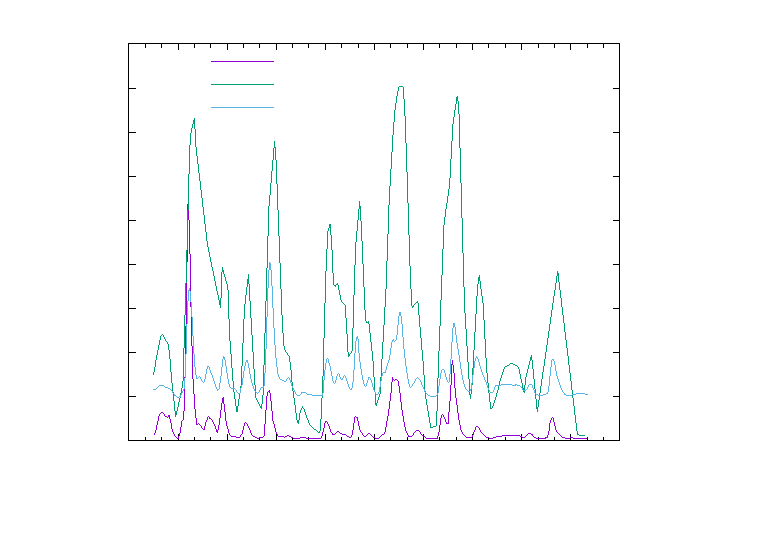
\includegraphics{../images/bus}}%
    \gplfronttext
  \end{picture}%
\endgroup

  \caption{Timeseries of the uncorrected \ch{NO2}, \ch{NO_x} and \ch{CO2}
    concentrations in the plume of a bus in Heidelberg.}
  \label{fig:bus-ts}
\end{figure}

Another interesting vehicle we pursued was a public-transit bus. We
followed it for \SI{10}{\minute} through mostly suburban areas with
almost no traffic. Therefore the values depicted in the timeseries in
Figure~\ref{fig:bus-ts} should give a rather pure picture of the bus's
emission. During our pursuit the bus stopped at 6 bus stops, which
explains the many acceleration periods depicted in the time
series. The missing ones are due to crossroads and traffic lights. As
before in the Mercedes case, we see that the \ch{NO_x} concentration
is the most volatile and the \ch{CO2} curve follows it in the same
general form. The \ch{NO2} concentration is the most stable, but shows
still a peak of over \SI{2500}{ppb} \ch{NO2}. In absolute terms, we
see that the bus has a factor 2 to 3 higher \ch{NO_x} emission peaks
thant the Mercedes. During the short periods of time in between bus
stops, the emission drops drastically and is in a comparable range to
the valleys in the Mercedes time series, however, since there are so
many bus stops in the route the emission during acceleration make up
the major part of the pollution. Looking at the ratios in
Table~\ref{tab:mercedes-bus}, we see that the bus has a three times
higher \ch{NO2} ratio, but the \ch{NO_x} ratio does not differ too
much. This can be explained by realizing that the bus naturally has a
far higher consumption than a normal street car. This directly leads
to higher emissions, especialle higher \ch{CO2} emissions, which
cancel out the larger Nitrogen (Di-)Oxide values. 

All in all these measurements yield two important take home
messages. First of all, we have further evidence that our converter
really works and that it produces additional detectable \ch{NO2} in
the cavity. An interesting question for further investigation would be
to find out, whether the converter was fast enough to complete convert
the whole \ch{NO} peaks. Dealing with \ch{NO_x} in the order of
magnitude of ppm (as in the Bus case), we could run in a region where
the Ozone concentration cannot be assumed to be constant anymore and
the reaction speed should diminish. Since we do not know the
conversion ratio for such high concentrations, the above \ch{NO_x}
values should be handled with care and be understood as a lower bound
for the emission. In any case, the second important message is, that
portable \ch{NO} measurement instruments are important for in vivo
vehicle measurements, as pure \ch{NO2} instruments may underestimate
the \ch{NO_x} emission by a factor 10. 

%%% Local Variables:
%%% mode: latex
%%% TeX-master: "../Bachelor"
%%% End:
